\section{Results}
\label{sec:results}

\begin{table}[t]
  \centering
  \small
  \setlength{\tabcolsep}{3.2pt}
  \resizebox{\linewidth}{!}{\begin{tabular}{lcccccc}
\toprule
 & \multicolumn{3}{c}{Qwen3-VL-8B} & \multicolumn{3}{c}{Qwen2.5-VL-7B} \\
\cmidrule(lr){2-4}\cmidrule(lr){5-7}
Second input & View & Swap & Stab. & View & Swap & Stab. \\
\midrule
Original image only & 48.5 & 31.0 & 65.5 & 48.0 & 32.5 & 50.0 \\
+ describe the change in text$^\dagger$ & 61.0 & \textbf{64.0} & 52.0 & 56.0 & 38.0 & 46.5 \\
+ own imagined state & 52.0 & 36.0 & 55.0 & 52.5 & 37.0 & 46.5 \\
+ oracle imagined state & \textbf{78.5} & 51.5 & \textbf{93.0} & \textbf{76.0} & \textbf{51.5} & \textbf{80.0} \\
+ another question's state & 50.0 & 34.5 & 54.0 & 49.5 & 28.0 & 49.5 \\
\midrule
+ misleading imagined state & 19.5 & 35.5 & 19.5 & 24.5 & 34.5 & 42.5 \\
\quad \emph{answers as the misleading state implies} & 80.5 & 28.0 & 80.5 & 75.5 & 36.5 & 57.5 \\
\bottomrule
\end{tabular}
}
  \caption{\textbf{Accuracy (\%) by second input}, 200 questions per task (chance: 50 / 29 / 50). Img.: original image only. Text: describe the change in words first. Own: the model's own imagined state. Oracle: the exact imagined state. Unrel.: another question's imagined state. Misl.: a misleading imagined state. Follows: how often the model gives the answer the misleading state implies. Best per row in bold (excluding Misl.). $^\dagger$Fewer questions (100--200 per task) for Text.}
  \label{tab:main}
\end{table}

\paragraph{Perfect imagination helps.} The oracle imagined state raises accuracy on every task for all three models (\cref{tab:main}): by 20--30 points for the two Qwen models and by 8--11 points for InternVL3-8B. All nine gains are significant (exact McNemar test, Holm-corrected over all comparisons, $p<0.05$; supplementary). An unrelated imagined state stays within 5 points of the image-only baseline, or lowers it (Qwen3-VL-8B, physical outcome: 65.5\,$\rightarrow$\,54.0), so the gain comes from the content of the image, not from a second image as such. The benefit also needs a model that can read the imagined state: the smaller Qwen2.5-VL-3B is near chance even on the imagined view alone (viewpoint: 52.5\%), and gains little from the oracle (47.5\,$\rightarrow$\,55.5). The pattern is unchanged under a paraphrased prompt with the options reversed (supplementary).

\paragraph{The model uses the imagined state.} A misleading imagined state lowers viewpoint accuracy below the image-only baseline for all three models (Qwen3-VL-8B 48.5\,$\rightarrow$\,19.5, Qwen2.5-VL-7B 48.0\,$\rightarrow$\,24.5, InternVL3-8B 51.0\,$\rightarrow$\,37.0, all significant), and the models then give the answer the misleading state implies 63--81\% of the time. Qwen3-VL-8B shows the same on physical outcome (65.5\,$\rightarrow$\,19.5; follows 80.5\%). The visual intermediate state therefore plays a causal role. The effect is weaker or absent where the image is harder to read (rearrangement) or where the model mostly ignores it (InternVL3-8B on physical outcome, which answers ``falls over'' for nearly every stack whenever a second image is given).

\paragraph{The seen image competes with the imagined one.} With the original image only, all three models answer viewpoint questions from their current view: accuracy is 78--99\% when the answer does not change after moving but 3--19\% when it does, matching the egocentric bias reported by Wang \etal~\cite{wang2026egocentric}. Given the imagined view \emph{alone}, they solve these hard cases (90--98\%). Given both images, they fall back to 61\% (Qwen3-VL-8B), 53\% (Qwen2.5-VL-7B) and 29\% (InternVL3-8B): the original image pulls the answer back towards the current view, by a different amount for each model. A method that produces a visual intermediate state must therefore also get the model to rely on it.

\paragraph{When does text reasoning suffice?} Describing the change in words first (``Text''; for Qwen3-VL-8B a mean of 646 generated tokens per answer, median 461, against at most 5 otherwise) gives a significant gain in one case only: Qwen3-VL-8B on rearrangement (31.0\,$\rightarrow$\,61.5), where it matches the oracle (51.5; difference not significant). Its reasoning rewrites ``closest to A after A and B trade places'' as ``closest to B's current position, apart from A'', which can be read from the original image without imagining anything. For viewpoint and physical outcome, no model gains significantly from text, while the oracle helps every model. Text suffices when a question can be re-expressed in terms of the visible scene; otherwise the imagined state is what helps.

\paragraph{How faithful must imagination be?} \Cref{fig:noise} adds Gaussian noise to every object's position before rendering the oracle (Qwen models). Viewpoint and rearrangement are forgiving: with $\sigma{=}1$\,m, Qwen3-VL-8B still reaches 70.0 and 41.0, above its image-only 48.5 and 31.0 (Qwen2.5-VL-7B: 67.0 and 39.5 vs.\ 48.0 and 32.5). Physical outcome is fragile, and accuracy follows how often the noisy state still implies the right outcome, falling to chance by $\sigma{=}0.5$\,m.

\begin{figure}[t]
  \centering
  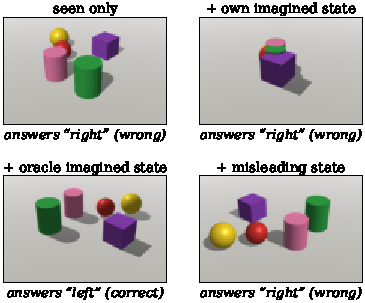
\includegraphics[width=\linewidth]{figs/qual.pdf}
  \caption{\textbf{One question, four second images} (Qwen3-VL-8B, actual answers). ``Walk a quarter turn to your right: is the green cylinder left or right of the red sphere?'' (answer: left). The model's own imagined state piles the objects together, so it does not help; the oracle does, and the misleading state flips the answer back.}
  \label{fig:qual}
\end{figure}

\paragraph{The model's own imagination is limited by perception.} When the model writes the scene down and we render the change, accuracy does not change significantly from the image-only baseline for any model or task (\cref{tab:main}, ``Own''; \cref{fig:qual}). Its reconstruction is worse than an oracle perturbed by 1\,m of noise (Qwen3-VL-8B, viewpoint: 52.0 vs.\ 70.0), because its errors are not random: it implies the correct viewpoint answer only 65\% of the time, and rescaling its layout to the true scene size does not change that (66\%). The failure is perception, not reasoning. On physical outcome, Qwen3-VL-8B answers correctly 96\% of the time when its own reconstruction implies the right outcome and 7.5\% when it does not, following its imagined state 94.5\% of the time, but its reconstruction is right only 53.5\% of the time.
